\documentclass[a4paper,12pt]{article}
\usepackage[english,russian]{babel}
\usepackage{graphicx}
\usepackage[utf8]{inputenc}
\usepackage[T2A]{fontenc}
\usepackage{amssymb,amsfonts,amsmath,cite,enumerate,float,indentfirst} %пакеты расширений
\usepackage{pgfplots}
\pgfplotsset{compat=1.9}
\usepackage{tikz}  
\usetikzlibrary{graphs}

\graphicspath{ {\картинки} }

\usepackage{geometry} % Меняем поля страницы
\geometry{left=2cm}% левое поле
\geometry{right=1.5cm}% правое поле
\geometry{top=1cm}% верхнее поле
\geometry{bottom=2cm}% нижнее поле

\title{Отчет по лабораторной работе "Корни уравнения"}
\author{Студент группы А-07-22 Татарников Максим}
\date{НИУ МЭИ 2023}
\begin{document}

\maketitle
\tableofcontents

\newpage

\section{Задание}

Методом деления отрезка пополам и методом хорд для N значений погрешности $\varepsilon$\\ $(0,1; 0,01;0,001;..1e-N, 1 \leq N \leq 10)$ вычислить значение корня для двух заданных функций №4 и №7 на отрезке $[A, B] \subset (0,2)$ и вывести их в виде таблицы (для каждой функции отдельную).

При вводе значений анализировать аномалии: $A, B, N$ – числа и $0<A<B<2, 1 \leq N \leq 10$.
Перед поиском корня обязательно проверять наличие корня на отрезке [A, B]
(разные знаки значения функции на концах отрезка).

Для самопроверки: 1) для каждой функции указан примерный корень для проверки
написания заданной функции, и 2) корни, найденные разными методами с одинаковой
точностью не должны отличаться больше, чем на эту точность.


\section{Функции}
\begin{equation}
f_1(x) = 1.5 - \frac{\sqrt{x} + \sqrt[3]{x}}{e^{3/2}} - x
\end{equation}
\begin{equation}
f_2(x) = 0.5(2-\sin{\frac{1+x}{x}} + \frac{1}{2}\ln{\sqrt{x}}) - x
\end{equation}

\section{Методы}

\subsection{Деление отрезка пополам}

\subsubsection{Описание метода}

Рисунок \ref{fig:method_half} иллюстрирует метод половинного деления, который состоит в постепенном сужении
отрезка поиска корня до заданной величины $\varepsilon$. На каждом шаге отрезок уменьшается вдвое. 

\begin{figure}[h]
\centering
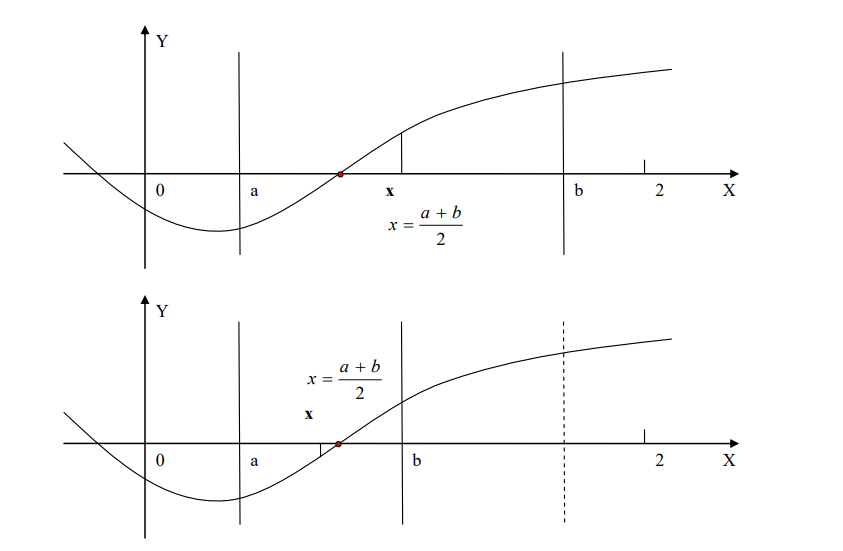
\includegraphics[scale=0.3]{отрезок_пополам.png}
\caption{Метод деление отрезка пополам}
\label{fig:method_half}
\end{figure}

В начале каждой итерации находим середину нового отрезка $[a , b]$

$$x = \frac{a+b}{2}$$

Затем следует определить, с какой стороны от середины отрезка $x$ находится корень $x*$. Для этого достаточно сравнить знаки $f (x)$ и $f (b)$ или знаки $f (x)$ и $f (a)$.

Если знаки $f (x)$ и $f (b)$ не совпадают, то это означает, что $f (x)$ пересекает ось $x$ на правом полуотрезке $[x, b]$. Следовательно, корня нет на левом полуотрезке $[a, x]$, и этот полуотрезок можно отбросить, то есть можно перенести левую границу $a$ в среднюю точку $x$ (заменить значение приближения $a$ на значение $x$).

Если же знаки $f (x)$ и $f (b)$ совпадают, то $f (x)$ пересекает ось $x$ на левом полуотрезке $[a, x]$ и, следовательно, корня нет на правом полуотрезке $[x ,b]$, и этот полуотрезок можно отбросить, то есть можно перенести правую границу $b$ в среднюю точку $x$ (заменить значение приближения $b$ на значение $x$).

Итак, в результате выполнения итерации отрезок $[a, b]$ как и прежде, содержит единственный корень, но его длина стала меньше в два раза.

Вычисления следует прекратить, если на очередном шаге длина отрезка $[a, b]$ станет меньше
$\varepsilon$. Тогда с точностью $\varepsilon$ любая точка этого отрезка будет являться корнем уравнения $f(x)$, а середина
этого отрезка – с точностью $\varepsilon/2$.
Совпадение знаков $f (x)$ и $f (b)$ можно проверить, проверив неравенство
$$f(x) \cdot f(b) > 0$$
поскольку произведение двух чисел с одинаковыми знаками дает положительное значение.

\subsubsection{Блок-схема}

\begin{figure}[h]
\centering
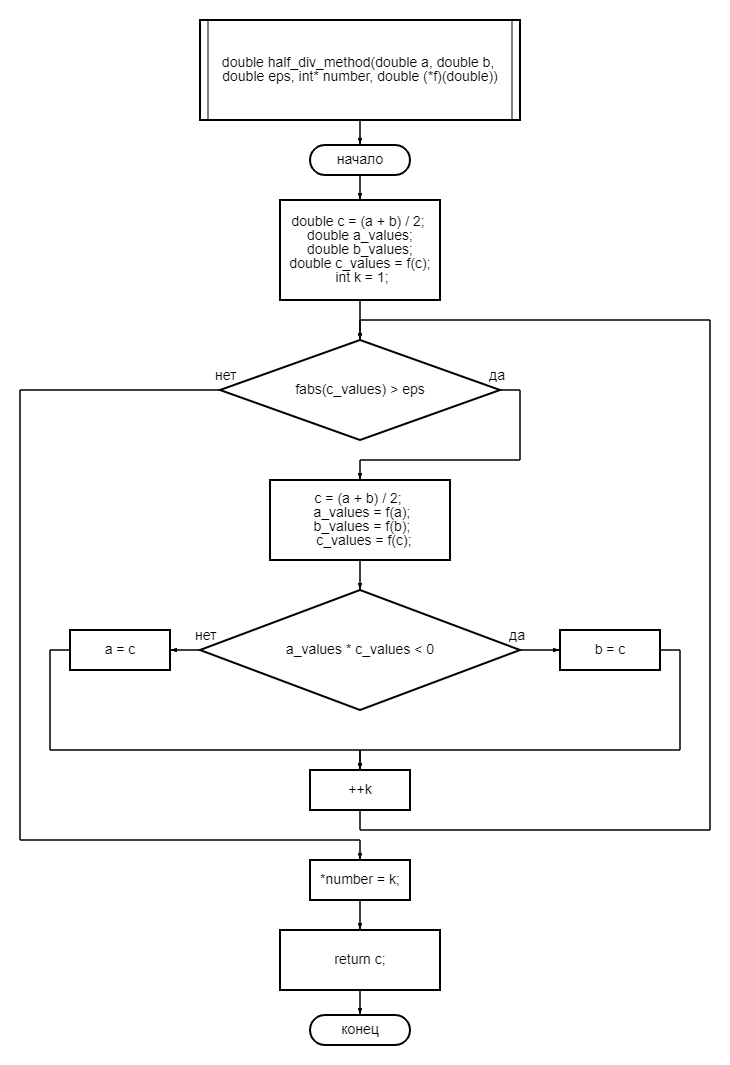
\includegraphics[scale=0.3]{diagram_half.png}
\caption{Метод деление отрезка пополам}
\label{fig:method_half_diagram}
\end{figure}

\newpage

\subsubsection{Программный код}

\begin{figure}[h]
\centering
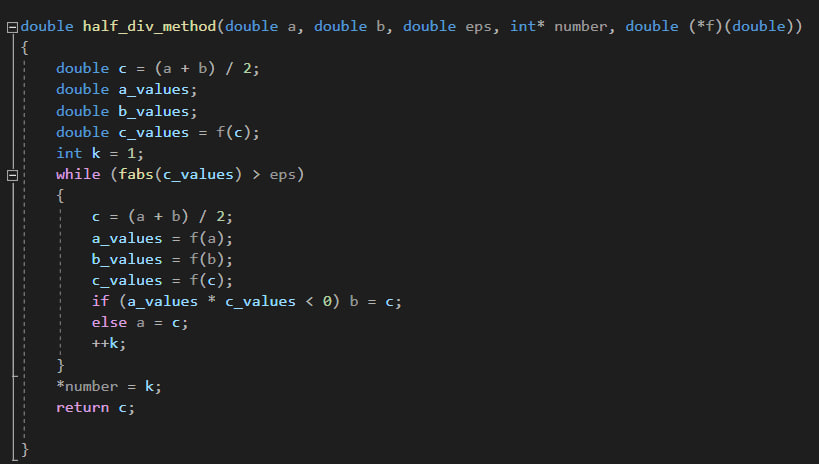
\includegraphics[scale=1]{отрезок_пополам.jpg}
\caption{Метод деление отрезка пополам}
\label{fig:method_half_code}
\end{figure}

\subsection{Метод хорд}

\subsubsection{Описание метода}
Этот метод вместе с методом бисекции относится к методам дихотомии – как отрезок делится
на две части, но на этот раз неравных. Точка деления отрезка находится как точка пересечения
отрезка, проведенного между точками $(a, f(a))$ и $(b, f (b))$, с осью $OX$ по формуле:



Новые значения $a$ и $b$ вычисляются так же, как и в методе бисекции – в зависимости от знаков
на границах новых отрезков $[a, x]$ и $[x, b]$. 

\begin{figure}[h]
\centering
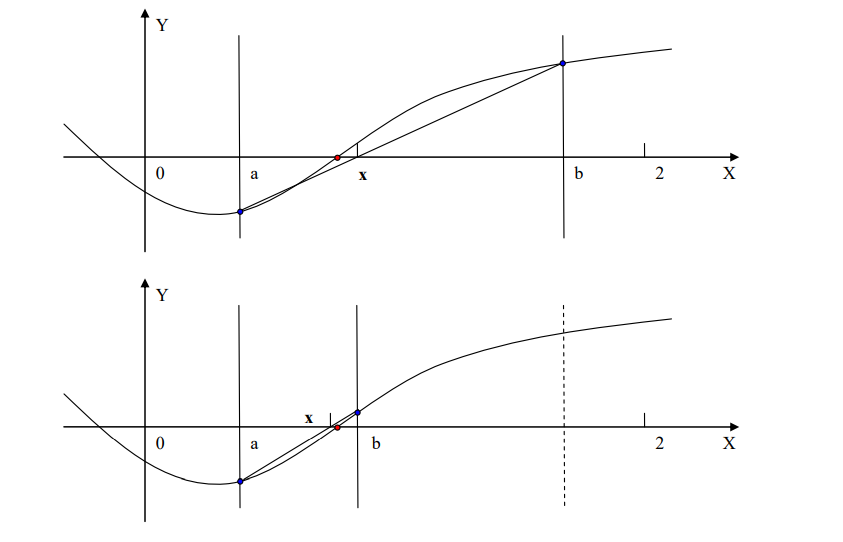
\includegraphics[scale=0.3]{хорд.png}
\caption{Метод хорд}
\label{fig:method_chord}
\end{figure}

При выполнении итераций по методу хорд может оказаться, что к корню приближается
только левая или только правая граница отрезка $[a, b]$. Поэтому в качестве меры близости к корню
здесь следует применить величину перемещения границы при очередной итерации, которая равна:

$$
        d=\begin{cases}
                 x - a, & \text{если корень справа от $x$ и перемещаем $a$,} \\
                 b - x, & \text{если корень слева от $x$ и перемещаем $b$.}
        \end{cases}
$$

Необходимая точность будет достигнута при выполнении после очередной итерации
неравенства:

$$|d| < \varepsilon $$

Полученное значение приближения x надо взять в качестве искомого значения корня.

\subsubsection{Блок-схема}

\begin{figure}[!h]
\centering
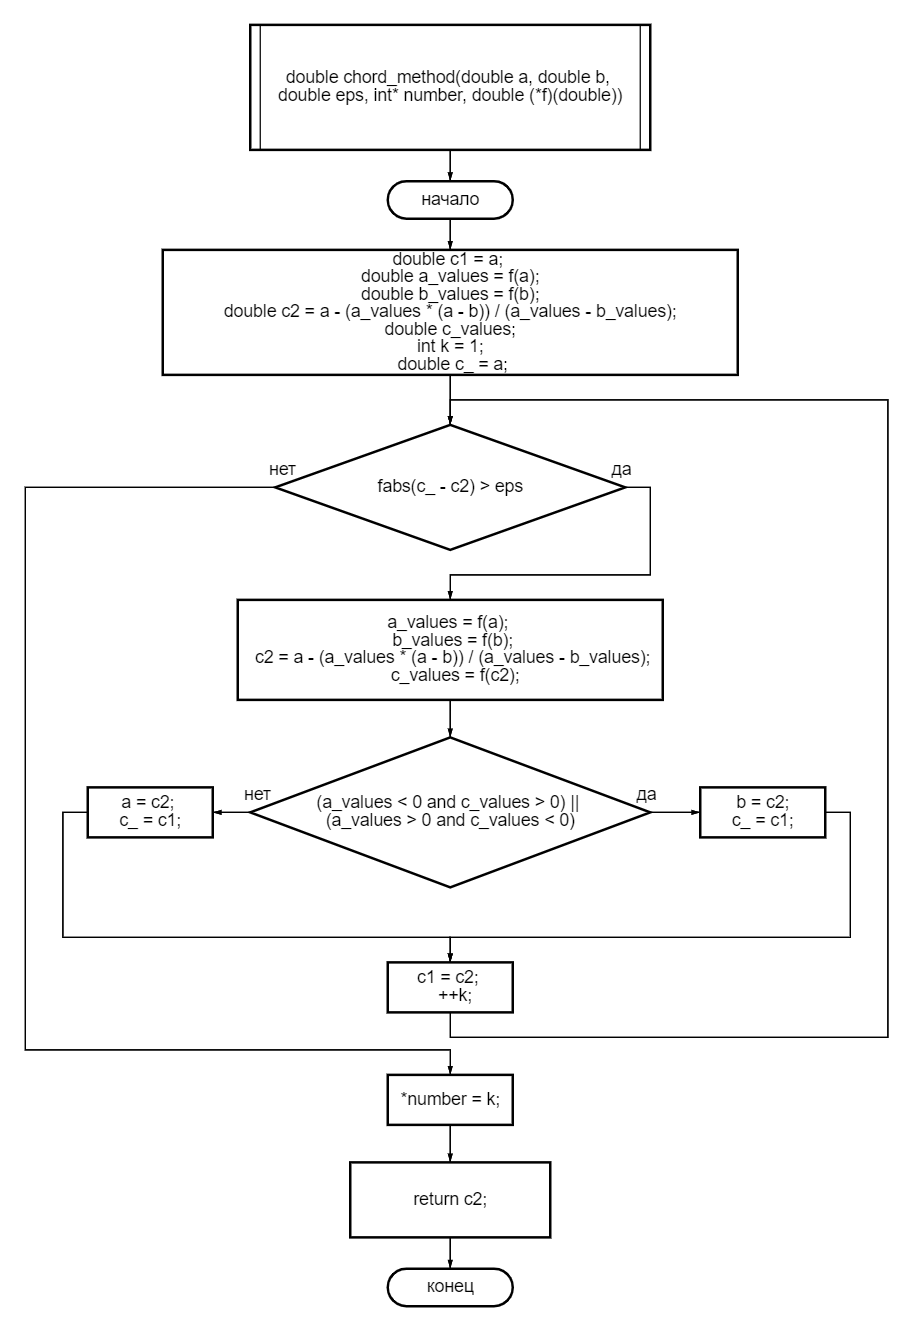
\includegraphics[scale=0.3]{diagram_chord.png}
\caption{Метод хорд}
\label{fig:method_chord_diagram}
\end{figure}

\newpage

\subsubsection{Программный код}

\begin{figure}[!h]
\centering
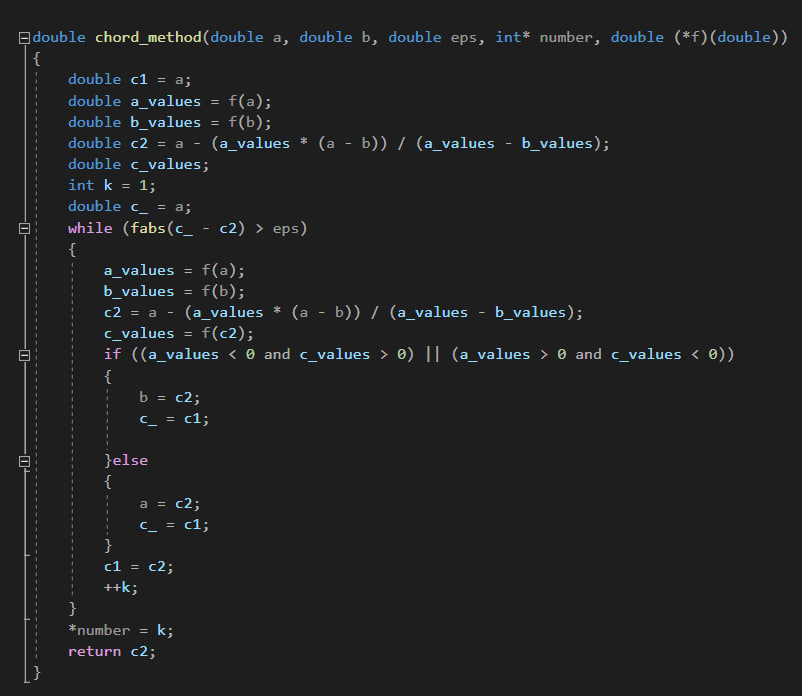
\includegraphics[scale=1]{хорд.jpg}
\caption{Метод хорд}
\label{fig:method_chord_code}
\end{figure}

\newpage

\subsection{Сравнение методов}

Различие двух методов состоит в том, что в случае деления отрезка пополам мы сравниваем значение функции с погрешность, а в методе хорд сравнение предыдущего и нового полученного аргумента, что напоминает предел последовательности, когда деление пополам - предел функции.

Сравним 2 метода:

\begin{figure}[!h]
\centering
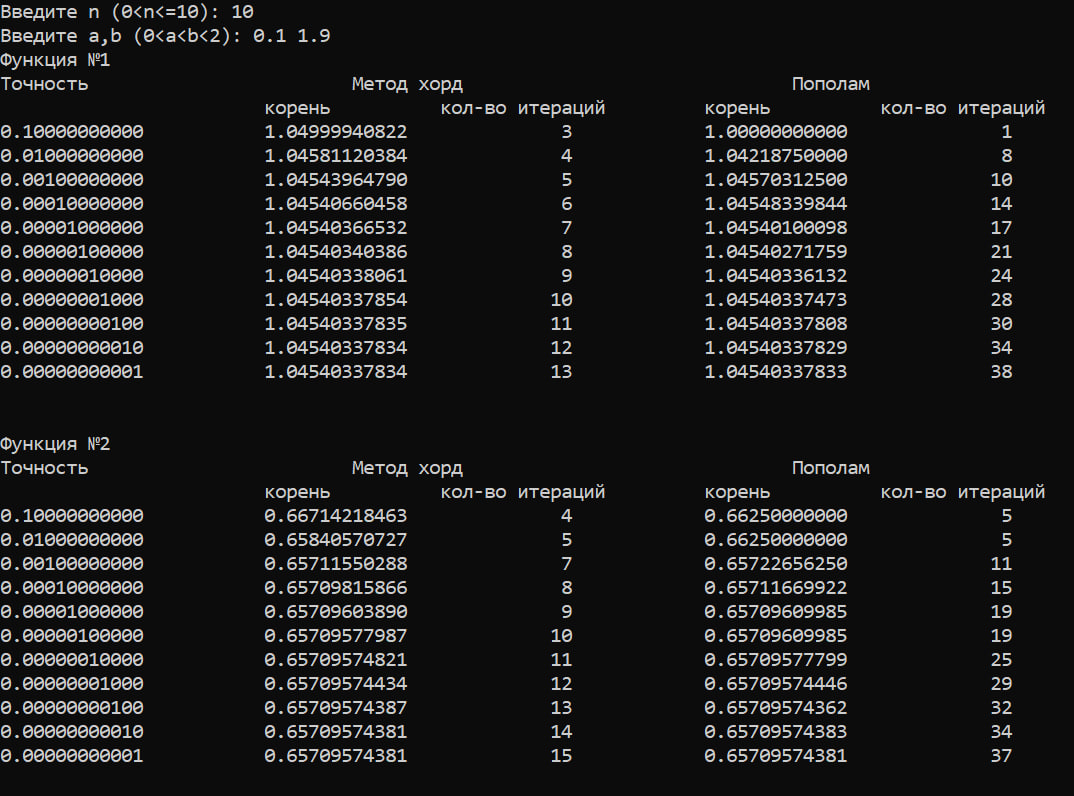
\includegraphics[scale=0.7]{таблица1.jpg}
\caption{Таблицы данных}
\label{fig:tab1}
\end{figure}

Не трудно заметить, что количество итераций в методе хорд $\sim2-2.5$ раза меньше, чем в методе деления отрезка пополам, из чего можно сделать вывод, что метод хорд эффективней.


\end{document}